\tikzset{every picture/.style={line width=0.75pt}} %set default line width to 0.75pt        
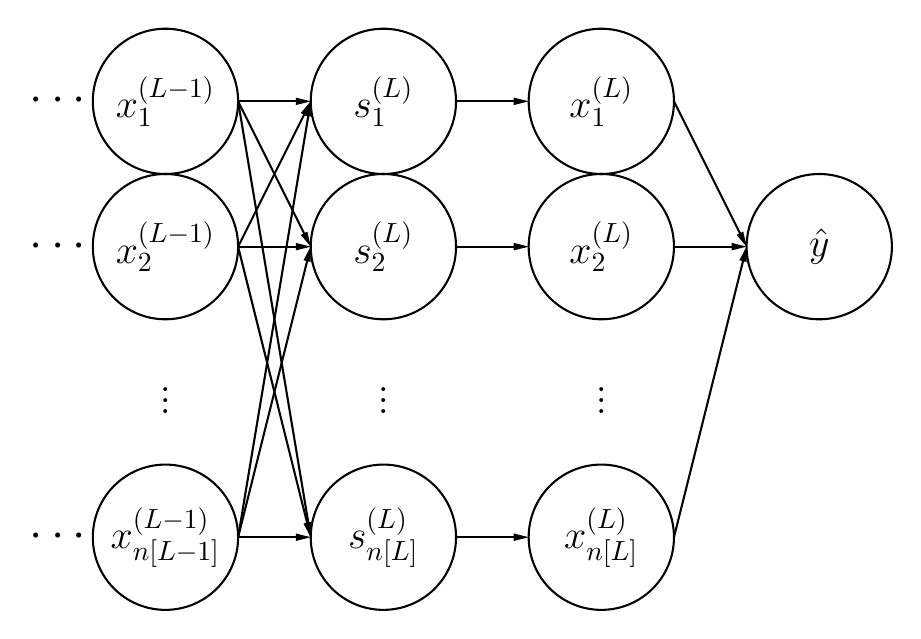
\begin{tikzpicture}[x=0.75pt,y=0.75pt,yscale=-1,xscale=1]
%uncomment if require: \path (0,301); %set diagram left start at 0, and has height of 301
%Shape: Circle [id:dp31498810996800775] 
\draw  [color={rgb, 255:red, 0; green, 0; blue, 0 }  ,draw opacity=1 ] (61,45) .. controls (61,25.67) and (76.67,10) .. (96,10) .. controls (115.33,10) and (131,25.67) .. (131,45) .. controls (131,64.33) and (115.33,80) .. (96,80) .. controls (76.67,80) and (61,64.33) .. (61,45) -- cycle ;
%Shape: Circle [id:dp5124453546700667] 
\draw  [color={rgb, 255:red, 0; green, 0; blue, 0 }  ,draw opacity=1 ] (61,115) .. controls (61,95.67) and (76.67,80) .. (96,80) .. controls (115.33,80) and (131,95.67) .. (131,115) .. controls (131,134.33) and (115.33,150) .. (96,150) .. controls (76.67,150) and (61,134.33) .. (61,115) -- cycle ;
%Shape: Circle [id:dp5314368935774948] 
\draw  [color={rgb, 255:red, 0; green, 0; blue, 0 }  ,draw opacity=1 ] (61,255) .. controls (61,235.67) and (76.67,220) .. (96,220) .. controls (115.33,220) and (131,235.67) .. (131,255) .. controls (131,274.33) and (115.33,290) .. (96,290) .. controls (76.67,290) and (61,274.33) .. (61,255) -- cycle ;
%Shape: Circle [id:dp8695451390182596] 
\draw  [color={rgb, 255:red, 0; green, 0; blue, 0 }  ,draw opacity=1 ] (166,45) .. controls (166,25.67) and (181.67,10) .. (201,10) .. controls (220.33,10) and (236,25.67) .. (236,45) .. controls (236,64.33) and (220.33,80) .. (201,80) .. controls (181.67,80) and (166,64.33) .. (166,45) -- cycle ;
%Shape: Circle [id:dp8391986584510998] 
\draw  [color={rgb, 255:red, 0; green, 0; blue, 0 }  ,draw opacity=1 ] (166,115) .. controls (166,95.67) and (181.67,80) .. (201,80) .. controls (220.33,80) and (236,95.67) .. (236,115) .. controls (236,134.33) and (220.33,150) .. (201,150) .. controls (181.67,150) and (166,134.33) .. (166,115) -- cycle ;
%Shape: Circle [id:dp28113471563872805] 
\draw  [color={rgb, 255:red, 0; green, 0; blue, 0 }  ,draw opacity=1 ] (166,255) .. controls (166,235.67) and (181.67,220) .. (201,220) .. controls (220.33,220) and (236,235.67) .. (236,255) .. controls (236,274.33) and (220.33,290) .. (201,290) .. controls (181.67,290) and (166,274.33) .. (166,255) -- cycle ;
%Straight Lines [id:da18284332414385995] 
\draw [color={rgb, 255:red, 0; green, 0; blue, 0 }  ,draw opacity=1 ]   (131,45) -- (164,45) ;
\draw [shift={(166,45)}, rotate = 180] [fill={rgb, 255:red, 0; green, 0; blue, 0 }  ,fill opacity=1 ][line width=0.08]  [draw opacity=0] (7.2,-1.8) -- (0,0) -- (7.2,1.8) -- cycle    ;
%Straight Lines [id:da6691579422613718] 
\draw [color={rgb, 255:red, 0; green, 0; blue, 0 }  ,draw opacity=1 ]   (131,115) -- (164,115) ;
\draw [shift={(166,115)}, rotate = 180] [fill={rgb, 255:red, 0; green, 0; blue, 0 }  ,fill opacity=1 ][line width=0.08]  [draw opacity=0] (7.2,-1.8) -- (0,0) -- (7.2,1.8) -- cycle    ;
%Straight Lines [id:da1847099123056497] 
\draw [color={rgb, 255:red, 0; green, 0; blue, 0 }  ,draw opacity=1 ]   (131,255) -- (164,255) ;
\draw [shift={(166,255)}, rotate = 180] [fill={rgb, 255:red, 0; green, 0; blue, 0 }  ,fill opacity=1 ][line width=0.08]  [draw opacity=0] (7.2,-1.8) -- (0,0) -- (7.2,1.8) -- cycle    ;
%Straight Lines [id:da7434606223833364] 
\draw [color={rgb, 255:red, 0; green, 0; blue, 0 }  ,draw opacity=1 ]   (131,255) -- (165.67,46.97) ;
\draw [shift={(166,45)}, rotate = 99.46] [fill={rgb, 255:red, 0; green, 0; blue, 0 }  ,fill opacity=1 ][line width=0.08]  [draw opacity=0] (7.2,-1.8) -- (0,0) -- (7.2,1.8) -- cycle    ;
%Straight Lines [id:da16747335923620488] 
\draw [color={rgb, 255:red, 0; green, 0; blue, 0 }  ,draw opacity=1 ]   (131,255) -- (165.51,116.94) ;
\draw [shift={(166,115)}, rotate = 104.04] [fill={rgb, 255:red, 0; green, 0; blue, 0 }  ,fill opacity=1 ][line width=0.08]  [draw opacity=0] (7.2,-1.8) -- (0,0) -- (7.2,1.8) -- cycle    ;
%Straight Lines [id:da5208262348209717] 
\draw [color={rgb, 255:red, 0; green, 0; blue, 0 }  ,draw opacity=1 ]   (131,45) -- (165.11,113.21) ;
\draw [shift={(166,115)}, rotate = 243.43] [fill={rgb, 255:red, 0; green, 0; blue, 0 }  ,fill opacity=1 ][line width=0.08]  [draw opacity=0] (7.2,-1.8) -- (0,0) -- (7.2,1.8) -- cycle    ;
%Straight Lines [id:da3798869604615329] 
\draw [color={rgb, 255:red, 0; green, 0; blue, 0 }  ,draw opacity=1 ]   (131,45) -- (165.67,253.03) ;
\draw [shift={(166,255)}, rotate = 260.54] [fill={rgb, 255:red, 0; green, 0; blue, 0 }  ,fill opacity=1 ][line width=0.08]  [draw opacity=0] (7.2,-1.8) -- (0,0) -- (7.2,1.8) -- cycle    ;
%Straight Lines [id:da9828802493660246] 
\draw [color={rgb, 255:red, 0; green, 0; blue, 0 }  ,draw opacity=1 ]   (131,115) -- (165.51,253.06) ;
\draw [shift={(166,255)}, rotate = 255.96] [fill={rgb, 255:red, 0; green, 0; blue, 0 }  ,fill opacity=1 ][line width=0.08]  [draw opacity=0] (7.2,-1.8) -- (0,0) -- (7.2,1.8) -- cycle    ;
%Straight Lines [id:da8792581248288048] 
\draw [color={rgb, 255:red, 0; green, 0; blue, 0 }  ,draw opacity=1 ]   (131,115) -- (165.11,46.79) ;
\draw [shift={(166,45)}, rotate = 116.57] [fill={rgb, 255:red, 0; green, 0; blue, 0 }  ,fill opacity=1 ][line width=0.08]  [draw opacity=0] (7.2,-1.8) -- (0,0) -- (7.2,1.8) -- cycle    ;
%Straight Lines [id:da050510950910013674] 
\draw    (341,45) -- (375.11,113.21) ;
\draw [shift={(376,115)}, rotate = 243.43] [fill={rgb, 255:red, 0; green, 0; blue, 0 }  ][line width=0.08]  [draw opacity=0] (7.2,-1.8) -- (0,0) -- (7.2,1.8) -- cycle    ;
%Straight Lines [id:da9492042893277386] 
\draw    (341,255) -- (375.51,116.94) ;
\draw [shift={(376,115)}, rotate = 104.04] [fill={rgb, 255:red, 0; green, 0; blue, 0 }  ][line width=0.08]  [draw opacity=0] (7.2,-1.8) -- (0,0) -- (7.2,1.8) -- cycle    ;
%Shape: Circle [id:dp7550531983138734] 
\draw   (376,115) .. controls (376,95.67) and (391.67,80) .. (411,80) .. controls (430.33,80) and (446,95.67) .. (446,115) .. controls (446,134.33) and (430.33,150) .. (411,150) .. controls (391.67,150) and (376,134.33) .. (376,115) -- cycle ;
%Straight Lines [id:da3526776996981338] 
\draw [color={rgb, 255:red, 0; green, 0; blue, 0 }  ,draw opacity=1 ]   (236,45) -- (269,45) ;
\draw [shift={(271,45)}, rotate = 180] [fill={rgb, 255:red, 0; green, 0; blue, 0 }  ,fill opacity=1 ][line width=0.08]  [draw opacity=0] (7.2,-1.8) -- (0,0) -- (7.2,1.8) -- cycle    ;
%Shape: Circle [id:dp0708162164794055] 
\draw   (271,45) .. controls (271,25.67) and (286.67,10) .. (306,10) .. controls (325.33,10) and (341,25.67) .. (341,45) .. controls (341,64.33) and (325.33,80) .. (306,80) .. controls (286.67,80) and (271,64.33) .. (271,45) -- cycle ;
%Straight Lines [id:da9789632975524958] 
\draw [color={rgb, 255:red, 0; green, 0; blue, 0 }  ,draw opacity=1 ]   (236,115) -- (269,115) ;
\draw [shift={(271,115)}, rotate = 180] [fill={rgb, 255:red, 0; green, 0; blue, 0 }  ,fill opacity=1 ][line width=0.08]  [draw opacity=0] (7.2,-1.8) -- (0,0) -- (7.2,1.8) -- cycle    ;
%Straight Lines [id:da9253632620657654] 
\draw [color={rgb, 255:red, 0; green, 0; blue, 0 }  ,draw opacity=1 ]   (236,255) -- (269,255) ;
\draw [shift={(271,255)}, rotate = 180] [fill={rgb, 255:red, 0; green, 0; blue, 0 }  ,fill opacity=1 ][line width=0.08]  [draw opacity=0] (7.2,-1.8) -- (0,0) -- (7.2,1.8) -- cycle    ;
%Shape: Circle [id:dp39051563534317957] 
\draw   (271,115) .. controls (271,95.67) and (286.67,80) .. (306,80) .. controls (325.33,80) and (341,95.67) .. (341,115) .. controls (341,134.33) and (325.33,150) .. (306,150) .. controls (286.67,150) and (271,134.33) .. (271,115) -- cycle ;
%Shape: Circle [id:dp3514602295749387] 
\draw   (271,255) .. controls (271,235.67) and (286.67,220) .. (306,220) .. controls (325.33,220) and (341,235.67) .. (341,255) .. controls (341,274.33) and (325.33,290) .. (306,290) .. controls (286.67,290) and (271,274.33) .. (271,255) -- cycle ;
%Straight Lines [id:da3353652086620188] 
\draw    (341,115) -- (374,115) ;
\draw [shift={(376,115)}, rotate = 180] [fill={rgb, 255:red, 0; green, 0; blue, 0 }  ][line width=0.08]  [draw opacity=0] (7.2,-1.8) -- (0,0) -- (7.2,1.8) -- cycle    ;

% Text Node
\draw (96,45) node  [font=\Large,color={rgb, 255:red, 0; green, 0; blue, 0 }  ,opacity=1 ]  {$x_{1}^{( L-1)}$};
% Text Node
\draw (96,115) node  [font=\Large,color={rgb, 255:red, 0; green, 0; blue, 0 }  ,opacity=1 ]  {$x_{2}^{( L-1)}$};
% Text Node
\draw (96,255) node  [font=\Large,color={rgb, 255:red, 0; green, 0; blue, 0 }  ,opacity=1 ]  {$x_{n[ L-1]}^{( L-1)}$};
% Text Node
\draw (201,45) node  [font=\Large,color={rgb, 255:red, 0; green, 0; blue, 0 }  ,opacity=1 ]  {$s_{1}^{( L)}$};
% Text Node
\draw (201,115) node  [font=\Large,color={rgb, 255:red, 0; green, 0; blue, 0 }  ,opacity=1 ]  {$s_{2}^{( L)}$};
% Text Node
\draw (201,255) node  [font=\Large,color={rgb, 255:red, 0; green, 0; blue, 0 }  ,opacity=1 ]  {$s_{n[ L]}^{( L)}$};
% Text Node
\draw (59,45) node [anchor=east] [inner sep=0.75pt]  [font=\LARGE,color={rgb, 255:red, 0; green, 0; blue, 0 }  ,opacity=1 ]  {$\cdots $};
% Text Node
\draw (59,115) node [anchor=east] [inner sep=0.75pt]  [font=\LARGE,color={rgb, 255:red, 0; green, 0; blue, 0 }  ,opacity=1 ]  {$\cdots $};
% Text Node
\draw (59,255) node [anchor=east] [inner sep=0.75pt]  [font=\LARGE,color={rgb, 255:red, 0; green, 0; blue, 0 }  ,opacity=1 ]  {$\cdots $};
% Text Node
\draw (96,185) node  [font=\LARGE,color={rgb, 255:red, 0; green, 0; blue, 0 }  ,opacity=1 ]  {$\vdots $};
% Text Node
\draw (201,185) node  [font=\LARGE,color={rgb, 255:red, 0; green, 0; blue, 0 }  ,opacity=1 ]  {$\vdots $};
% Text Node
\draw (411,115) node  [font=\Large]  {$\hat{y}$};
% Text Node
\draw (306,45) node  [font=\Large]  {$x_{1}^{( L)}$};
% Text Node
\draw (306,115) node  [font=\Large]  {$x_{2}^{( L)}$};
% Text Node
\draw (306,255) node  [font=\Large]  {$x_{n[ L]}^{( L)}$};
% Text Node
\draw (306,185) node  [font=\LARGE]  {$\vdots $};
\end{tikzpicture}